\documentclass[border=10pt]{standalone}
\usepackage{tikz}
\usetikzlibrary{positioning}
\tikzset{
  vertex/.style = {font = \sffamily\bfseries, text = white,
          shape = circle, ball color = blue},
  bridge/.style = {thick, double = yellow,
          double distance = 1pt},
  number/.style = {font = \sffamily\bfseries, text = white,
          draw, fill = red}}
\begin{document}
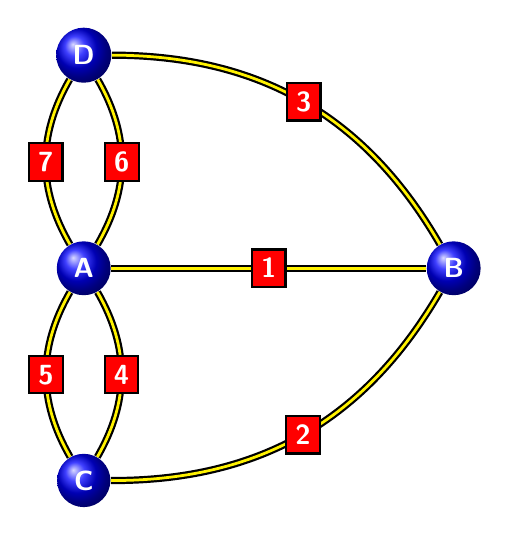
\begin{tikzpicture}
  \node[vertex] (A) {A};
  \node[vertex, right = 4 cm of A] (B) {B};
  \draw (A) edge [bridge] node [number] {1} (B);
  \node[vertex, below = 2cm of A] (C) {C};
  \node[vertex, above = 2cm of A] (D) {D};
  \tikzset{bridge/.append style = {bend right}}
  \draw (C) edge [bridge] node [number] {2} (B)
        (B) edge [bridge] node [number] {3} (D)
        (C) edge [bridge] node [number] {4} (A)
        (A) edge [bridge] node [number] {5} (C)
        (A) edge [bridge] node [number] {6} (D) 
        (D) edge [bridge] node [number] {7} (A);
\end{tikzpicture}
\end{document}
